% !TEX encoding = UTF-8 Unicode
\DocumentMetadata{
  lang = eng-US,
  pdfstandard = A-3u,
  pdfversion = 1.7,
}

\documentclass[colorlinks,upint,subscriptcorrection,varvw,balance,nofoot]{asmeconf}

\hypersetup{
  pdfauthor={Chance Lavoie},
  pdftitle={Eqn2Sim: Deterministic Compilation of Restricted LaTeX ODEs into Validated, Readable Simulink Models},
  pdfkeywords={deterministic compiler, Simulink, symbolic ODE, benchmark, model-based design},
  pdfsubject={ASME conference-style manuscript for the Eqn2Sim deterministic equation-to-Simulink compiler},
}

\usepackage{amsmath}
\usepackage{booktabs}
\usepackage{enumitem}
\usepackage{graphicx}
\usepackage{tabularx}
\usepackage{tikz}
\usetikzlibrary{arrows.meta,backgrounds,calc,fit,positioning}

\newcommand{\EqnToSim}{\NoCaseChange{Eqn2Sim}}

\begin{document}

\ConfName{ASME Conference Manuscript Draft}
\ConfAcronym{ASME-DRAFT}
\ConfDate{March 2026}
\ConfCity{Pittsburgh, PA}
\PaperNo{DRAFT-EQN2SIM}

\title{\EqnToSim: Deterministic Compilation of Restricted \NoCaseChange{\LaTeX} ODEs into Validated, Readable Simulink Models}

\SetAuthors{Chance Lavoie\affil{1}\CorrespondingAuthor{chancel@andrew.cmu.edu}}
\SetAffiliation{1}{Carnegie Mellon University, Pittsburgh, PA}

\maketitle

\versionfootnote{Draft manuscript prepared from the validated repository artifacts on \today.}

\keywords{deterministic compiler, Simulink, equation-based modeling, symbolic computation, benchmark, model-based design}

\begin{abstract}
Engineers often derive dynamics as equations first and rebuild block diagrams later by hand. That translation step is slow, error-prone, and difficult to validate. This paper presents \EqnToSim, a deterministic compiler that converts a restricted \LaTeX{} representation of ordinary differential equations into validated, human-readable Simulink models. The pipeline normalizes and parses \LaTeX{} into a canonical intermediate representation, deterministically classifies states, isolates highest-order derivatives, lowers explicit first-order systems into a shared-subexpression graph, and generates real \texttt{.slx} models through the MATLAB Engine API. A second backend layer adds deterministic layout, per-state subsystems, integrator-chain organization, and symbolic signal labels without changing numerical behavior. Across a 216-case synthetic benchmark and a 255-case full benchmark suite spanning verified, structural, and adversarial tiers, every case satisfied its benchmark criterion. For compared cases, the average root-mean-square error between Python and Simulink trajectories was $1.36\times10^{-11}$ and the worst observed maximum absolute error was $3.96\times10^{-9}$, both far below the $10^{-6}$ acceptance tolerance. Hard nonlinear coupled examples also produced valid Simulink models and matched reference ODE simulations.
\end{abstract}

\begin{nomenclature}
\EntryHeading{Acronyms}
\entry{CSE}{Common subexpression elimination}
\entry{IR}{Intermediate representation}
\entry{ODE}{Ordinary differential equation}
\entry{RMSE}{Root-mean-square error}
\end{nomenclature}

\section{Introduction}
Dynamic-system models often begin life as textbook-style equations, homework derivations, lab notes, or controller design memos. In many engineering workflows, those equations still must be manually translated into a block-diagram environment before the model can participate in simulation, verification, or code-generation activities. Simulink is a widely used graphical environment for hierarchical dynamic-system modeling, simulation, and model-based design \cite{mathworks2025simulink}. However, direct equation-to-diagram translation is usually manual.

This work targets that gap with a narrow but fully deterministic compiler. \EqnToSim{} accepts a restricted subset of \LaTeX{} ODE notation, compiles it into symbolic and graph-based internal forms, generates real Simulink models, simulates them through MATLAB, and validates the resulting trajectories against Python reference simulations. The system is intentionally strict: unsupported constructs fail explicitly instead of being guessed or heuristically repaired.

The project has two design goals. First, it must be numerically trustworthy, meaning that every generated model is checked against a reference ODE simulation and, when applicable, a derived state-space simulation. Second, the generated Simulink model must be readable enough for human inspection. To support the second goal, the current backend includes deterministic layout, per-state subsystem grouping, integrator-chain organization, and symbolic signal labels.

The main contributions of this paper are:
\begin{itemize}[leftmargin=*,nosep]
\item a deterministic compiler from restricted \LaTeX{} ODEs to canonical symbolic forms, explicit first-order systems, and Simulink-ready graphs;
\item a validated Simulink backend that builds real \texttt{.slx} models, runs them through MATLAB, extracts logged signals, and compares them to Python reference trajectories;
\item a readable second-generation backend that improves organization and signal traceability without changing numerical results; and
\item a research-grade benchmark suite, \NoCaseChange{SimuCompileBench}, that combines preserved synthetic coverage, harder structural systems, and explicitly categorized adversarial failures.
\end{itemize}

\section{Related Work}
Equation-oriented modeling languages such as Modelica showed early that physical-system behavior can be compiled from declarative equations instead of being hand-wired as block diagrams \cite{fritzson1998modelica}. OpenModelica extended that tradition with an integrated open-source environment for modeling, symbolic compilation, simulation, optimization, and model exchange \cite{fritzson2020openmodelica}. Work on bootstrapping the OpenModelica compiler also illustrates the depth and complexity of equation-based compilation pipelines \cite{sjolund2014bootstrapping}.

These systems are closely related to \EqnToSim{}, but the problem boundary is different. Modelica and OpenModelica are full modeling languages with large compilation stacks and broad acausal capabilities. \EqnToSim{} instead begins from a deliberately restricted \LaTeX{} notation that resembles how many engineers first write differential equations. The output target is not only an executable simulator state, but also an inspectable Simulink block diagram.

The implementation also relies on well-established symbolic and numerical infrastructure. SymPy provides the symbolic expression manipulation and structural comparison mechanisms used in the compiler pipeline \cite{meurer2017sympy}. SciPy provides the reference ODE integration path used for direct simulation and numerical validation \cite{virtanen2020scipy}. MATLAB and Simulink supply the block-diagram environment and the Python bridge used for model creation and execution \cite{mathworks2025simulink,mathworks2025python}. Future interoperability work can build on standards such as FMI \cite{fmi302}, but the present contribution is a deterministic equation-to-Simulink pipeline with explicit benchmark boundaries.

\section{Methods}
\subsection{Compiler Boundary and Deterministic Frontend}
\EqnToSim{} does not attempt to parse arbitrary \LaTeX. The accepted language is a deterministic subset consisting of newline-separated equations, derivative operators such as $\dot{x}$, $\ddot{x}$, and $\frac{d^n x}{dt^n}$, indexed variables such as $x_1$, nested fractions, implicit multiplication, selected transcendental functions, and algebraic operators. Unsupported syntax raises explicit compile errors.

After normalization, tokenization, and parsing, each equation is represented as typed expression nodes and a canonical dictionary IR. This representation removes formatting ambiguity while keeping enough structure to support deterministic state extraction, symbolic solving, graph lowering, and later traceability back to the source expressions.

\subsection{State Extraction, Canonicalization, and First-Order Realization}
The compiler classifies symbols into state candidates, derivative-derived states, inputs, and parameters using deterministic rules plus optional user-specified metadata. The highest-order derivatives are then isolated symbolically. Mixed-order systems are expanded into explicit first-order state chains, and linear systems additionally produce a state-space realization.

For example, the mass-spring-damper equation
\begin{align}
  m\ddot{x} + c\dot{x} + kx &= u
\end{align}
is converted into the first-order form
\begin{align}
  \dot{x} &= v \\
  \dot{v} &= \frac{u - cv - kx}{m}.
  \label{eq:massspring_first_order}
\end{align}
This explicit first-order system is the common numerical target for the Python simulation path, the graph-lowering path, and, when linear, the state-space branch.

\subsection{Graph Lowering and Simulink Generation}
The first-order system is lowered into a deterministic signal-dependency graph with stable node identifiers and structural CSE. Repeated subexpressions such as $\sin(\theta_1-\theta_2)$ are generated once and fanned out to all consumers. The graph supports constants, inputs, state signals, arithmetic operators, powers, selected transcendental functions, and integrators.

The Simulink backend maps graph operators to block-library elements. Integrators map to continuous-time Integrator blocks; sums map to Sum blocks; products, divisions, gains, and powers map to combinations of Product, Divide, Gain, and Math Function blocks; and trigonometric functions map to Simulink trigonometric-function blocks. Constant runtime values become Constant blocks, while time-varying inputs can be injected through workspace-backed source blocks. MATLAB Engine for Python is used to create the model, add blocks, connect wires, save the \texttt{.slx} file, run simulation, and extract logged outputs \cite{mathworks2025python}.

\subsection{Readable Backend v2}
The second-generation backend augments the validated numerical path with a presentation layer. Blocks are placed according to deterministic topological layers, organized into per-state subsystems, and arranged so that integrator chains visually expose the state evolution path:
\begin{align}
  x_{ddot} \rightarrow \int \rightarrow x_{dot} \rightarrow \int \rightarrow x.
\end{align}
The backend also propagates symbolic expressions to internal signals, allowing model wiring to retain human-readable meaning instead of anonymous connection names.

These visual improvements were developed as an isolated clone of the original backend and then regression-tested against the original pipeline. The resulting v2 backend preserved numerical equivalence on every curated comparison case while producing clearer hierarchical diagrams.

\subsection{Benchmark Design and Validation}
Benchmarking is organized into three tiers. Tier~1 preserves the original 216-case synthetic benchmark over supported state counts, expression depths, linear and nonlinear classes, and trig versus non-trig variants. Tier~2 adds harder structural systems, including 8-, 10-, and 12-state dense systems, higher-order families, controlled systems, and physical-inspired mass-spring and RC/RLC examples. Tier~3 contains adversarial cases designed to fail cleanly, including parse failures, symbolic dead ends, graph-invalid structures, and numerical-instability probes.

Each benchmark case is evaluated stage by stage: parse, state extraction, symbolic solve, first-order conversion, graph lowering, graph validation, Python simulation, Simulink build, Simulink simulation, and numerical comparison. A successful supported case must satisfy
\begin{align}
  \mathrm{RMSE} < 10^{-6}, \qquad \max |e(t)| < 10^{-6}.
\end{align}
An adversarial case is considered successful only if it fails at the intended stage with an explicit categorized error.

\begin{figure*}[t]
\centering
\resizebox{\textwidth}{!}{%
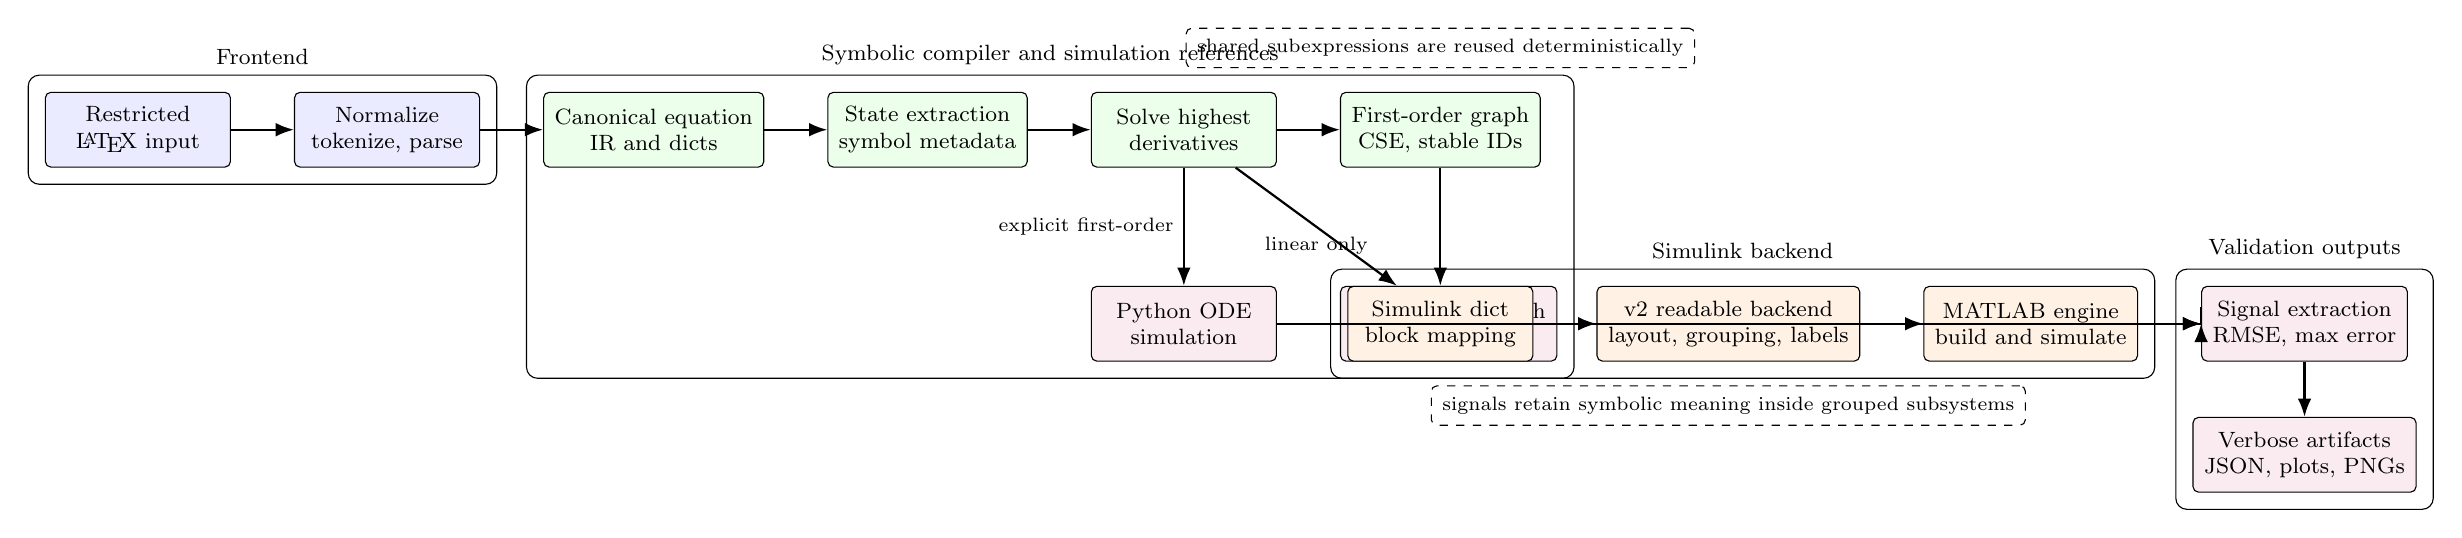
\begin{tikzpicture}[
  >=Latex,
  font=\footnotesize,
  node distance=7mm and 8mm,
  stage/.style={draw, rounded corners=2pt, align=center, minimum width=2.35cm, minimum height=0.95cm, inner sep=4pt},
  frontend/.style={stage, fill=blue!8},
  core/.style={stage, fill=green!8},
  backend/.style={stage, fill=orange!10},
  validate/.style={stage, fill=purple!8},
  outline/.style={draw, rounded corners=4pt, inner sep=6pt},
  line/.style={->, thick},
  labelbox/.style={draw, dashed, rounded corners=2pt, fill=white, inner sep=4pt, font=\scriptsize}
]
  \node[frontend] (latex) {Restricted\\\LaTeX{} input};
  \node[frontend, right=of latex] (parse) {Normalize\\tokenize, parse};
  \node[core, right=of parse] (ir) {Canonical equation\\IR and dicts};
  \node[core, right=of ir] (symbols) {State extraction\\symbol metadata};
  \node[core, right=of symbols] (solve) {Solve highest\\derivatives};
  \node[core, right=of solve] (graph) {First-order graph\\CSE, stable IDs};

  \node[validate, below=15mm of solve] (ode) {Python ODE\\simulation};
  \node[validate, right=of ode] (ss) {State-space branch\\when linear};

  \node[backend, below=15mm of graph] (sdict) {Simulink dict\\block mapping};
  \node[backend, right=of sdict] (layout) {v2 readable backend\\layout, grouping, labels};
  \node[backend, right=of layout] (builder) {MATLAB engine\\build and simulate};
  \node[validate, right=of builder] (compare) {Signal extraction\\RMSE, max error};
  \node[validate, below=of compare] (reports) {Verbose artifacts\\JSON, plots, PNGs};

  \draw[line] (latex) -- (parse);
  \draw[line] (parse) -- (ir);
  \draw[line] (ir) -- (symbols);
  \draw[line] (symbols) -- (solve);
  \draw[line] (solve) -- (graph);
  \draw[line] (graph) -- (sdict);
  \draw[line] (sdict) -- (layout);
  \draw[line] (layout) -- (builder);
  \draw[line] (builder) -- (compare);
  \draw[line] (compare) -- (reports);

  \draw[line] (solve) -- node[left, font=\scriptsize] {explicit first-order} (ode);
  \draw[line] (solve) -- node[below, font=\scriptsize] {linear only} (ss);
  \draw[line] (ode.east) -| (compare.west);
  \draw[line] (ss.east) |- (compare.west);

  \node[labelbox, above=3mm of graph] (cse) {shared subexpressions are reused deterministically};
  \node[labelbox, below=3mm of layout] (trace) {signals retain symbolic meaning inside grouped subsystems};

  \node[outline, fit=(latex)(parse), label=above:{Frontend}] {};
  \node[outline, fit=(ir)(symbols)(solve)(graph)(ode)(ss), label=above:{Symbolic compiler and simulation references}] {};
  \node[outline, fit=(sdict)(layout)(builder), label=above:{Simulink backend}] {};
  \node[outline, fit=(compare)(reports), label=above:{Validation outputs}] {};
\end{tikzpicture}
}
\caption{Eqn2Sim architecture. Restricted \LaTeX{} equations are normalized into canonical symbolic forms, lowered into a reusable graph, compiled into a real Simulink model, and validated against Python reference simulations. The v2 backend adds deterministic layout, subsystem grouping, integrator-chain clarity, and symbolic signal traceability without changing the numerical path.}
\label{fig:pipeline}
\end{figure*}

\section{Results}
\subsection{Benchmark Coverage}
Table~\ref{tab:tiers} summarizes the benchmark structure. Every case satisfied its benchmark criterion. Importantly, the 11 adversarial cases were counted as benchmark passes only because they failed cleanly and at the expected stage. No silent failures remained in the benchmark reports.

\begin{table}[t]
\caption{Tiered benchmark summary for \NoCaseChange{SimuCompileBench}.}
\label{tab:tiers}
\centering
\begin{tabularx}{\columnwidth}{@{}l c X c@{}}
\toprule
Tier & Systems & Purpose & Result \\
\midrule
Tier 1 verified & 216 & Preserved synthetic benchmark across supported linear and nonlinear ODE families & 216/216 \\
Tier 2 structural & 28 & Higher-order, controlled, scaled, and physical-inspired systems & 28/28 \\
Tier 3 adversarial & 11 & Expected failures, graph faults, and instability probes & 11/11 \\
\midrule
Total & 255 & Full benchmark suite & 255/255 \\
\bottomrule
\end{tabularx}
\end{table}

Across compared cases in the full benchmark, the average RMSE between Python and Simulink trajectories was $1.36\times10^{-11}$, the average maximum absolute error was $6.49\times10^{-11}$, and the worst observed maximum absolute error was $3.96\times10^{-9}$. All of these values remained well below the acceptance threshold of $10^{-6}$. The explicit failure categories observed in the adversarial tier were four parse failures, five symbolic failures, one graph-invalid case, and one numerical-instability case.

\subsection{Scaling on the Preserved Synthetic Suite}
The legacy 216-case synthetic suite remained fully intact after the backend cleanup and readable-layout integration. Table~\ref{tab:scaling} shows how graph size, Simulink block count, and build time scaled with generated state count on that preserved benchmark.

\begin{table}[t]
\caption{Scaling on the preserved 216-case synthetic benchmark.}
\label{tab:scaling}
\centering
\footnotesize
\begin{tabularx}{\columnwidth}{@{}c c c c@{}}
\toprule
States & Avg. graph & Avg. blocks & Build [s] \\
\midrule
1 & 12.83 & 14.72 & 2.47 \\
2 & 22.47 & 29.86 & 2.77 \\
3 & 31.44 & 44.81 & 3.27 \\
4 & 37.39 & 56.67 & 3.66 \\
5 & 44.69 & 70.56 & 3.93 \\
6 & 51.36 & 83.00 & 4.12 \\
\bottomrule
\end{tabularx}
\end{table}

Average simulation time on this suite remained near $0.18$~s per case. The readable backend therefore did not prevent the system from scaling through the original benchmark while preserving the published pass rate of 216/216.

\subsection{Readable Backend Equivalence}
The second-generation readable backend was also compared directly against the original backend on nine curated examples. All nine matched numerically, and all six Simulink-backed examples in that set retained their reference behavior. This regression set established that subsystem grouping, signal labels, and layout heuristics were additive presentation improvements rather than mathematical changes.

\subsection{Hard Nonlinear Examples}
The benchmark suite also includes harder nonlinear systems that stress coupled trigonometric terms, higher-order derivatives, and nonlinear accelerations. Table~\ref{tab:hardexamples} summarizes representative cases that passed the full nonlinear Simulink path. These systems do not rely on the linear state-space branch; instead, the generated Simulink model is compared directly against the Python ODE simulation.

\begin{table}[t]
\caption{Representative hard nonlinear systems that passed the full ODE-to-Simulink validation path.}
\label{tab:hardexamples}
\centering
\footnotesize
\begin{tabularx}{\columnwidth}{@{}X c c c@{}}
\toprule
Example & States & RMSE & Max abs. error \\
\midrule
Cart-pendulum-spring & 4 & $1.23\times10^{-9}$ & $2.12\times10^{-8}$ \\
Coupled trig difference & 4 & $2.88\times10^{-10}$ & $8.76\times10^{-10}$ \\
Nested nonlinear & 2 & $4.88\times10^{-10}$ & $6.76\times10^{-9}$ \\
Third-order nonlinear & 3 & $1.91\times10^{-9}$ & $1.67\times10^{-8}$ \\
Double-pendulum pair & 4 & $1.16\times10^{-10}$ & $2.58\times10^{-10}$ \\
\bottomrule
\end{tabularx}
\end{table}

Figure~\ref{fig:cartpendulum} shows one of these nonlinear cases: a coupled cart-pendulum-spring system with nonzero initial conditions. The readable backend groups the generated model into state-specific subsystems and preserves symbolic structure on the internal wiring, while the numerical comparison shows that the Simulink and ODE trajectories overlap at plotting resolution.

\begin{figure*}[t]
\centering
\begin{minipage}[t]{0.34\textwidth}
\centering
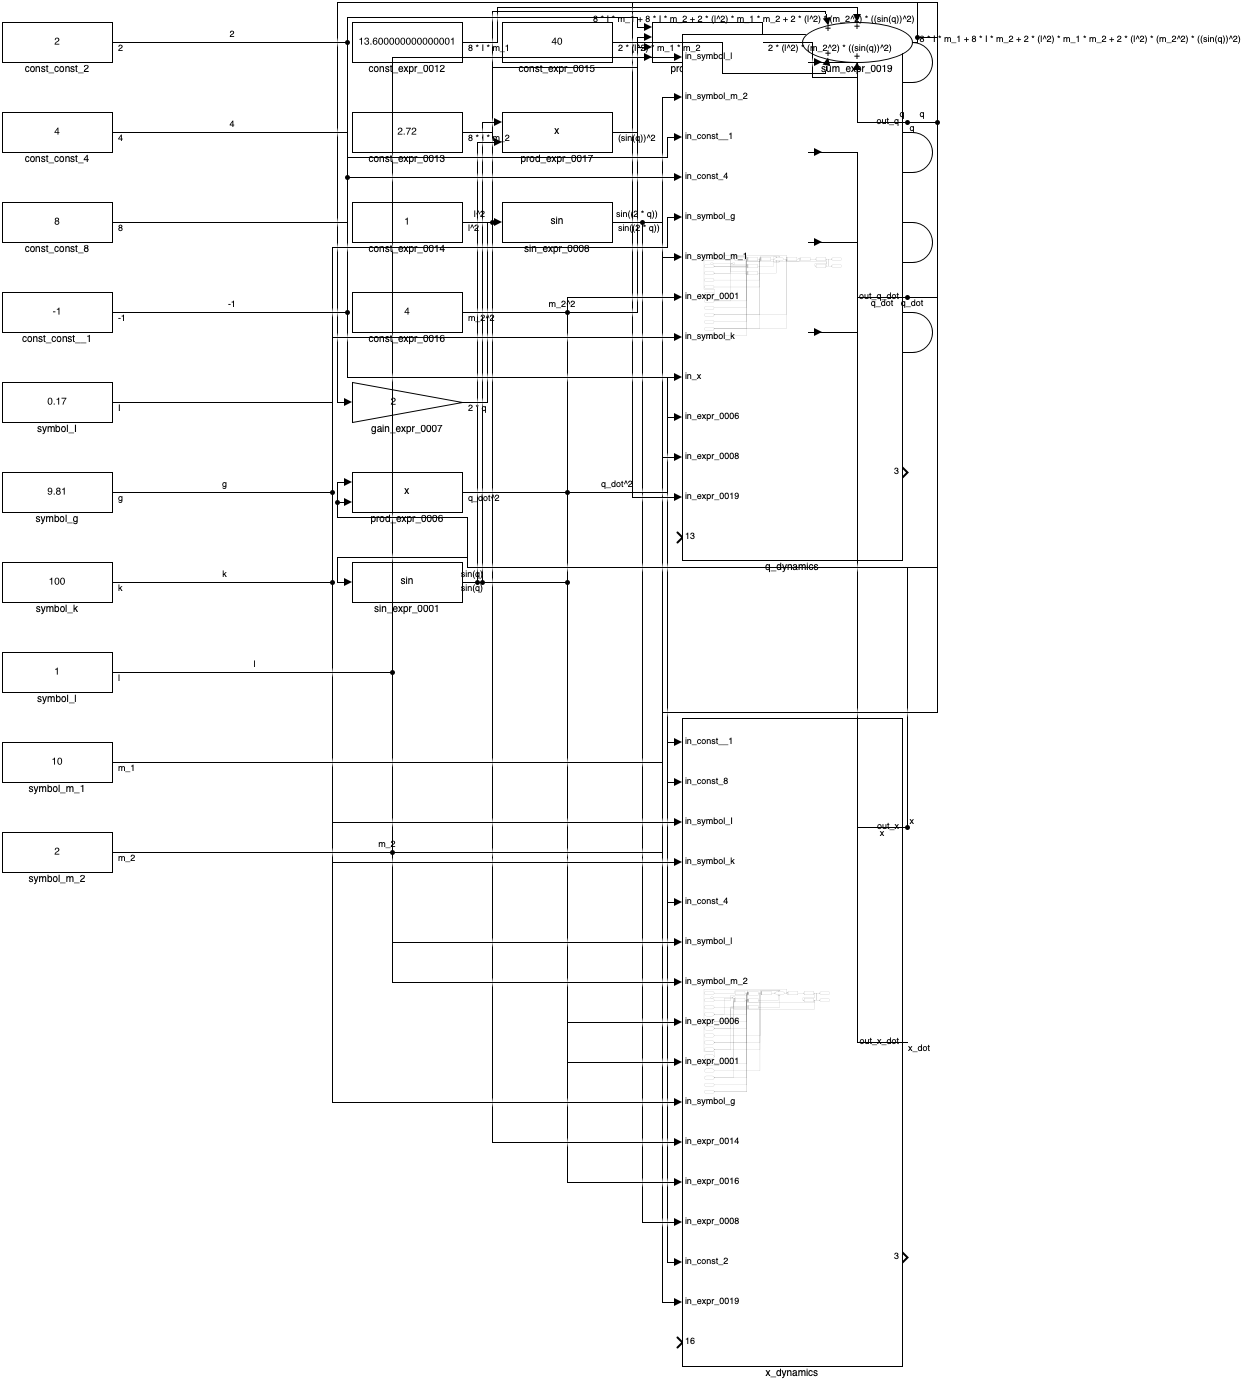
\includegraphics[width=\linewidth]{figures/cart_pendulum_model.png}
\end{minipage}\hfill
\begin{minipage}[t]{0.63\textwidth}
\centering
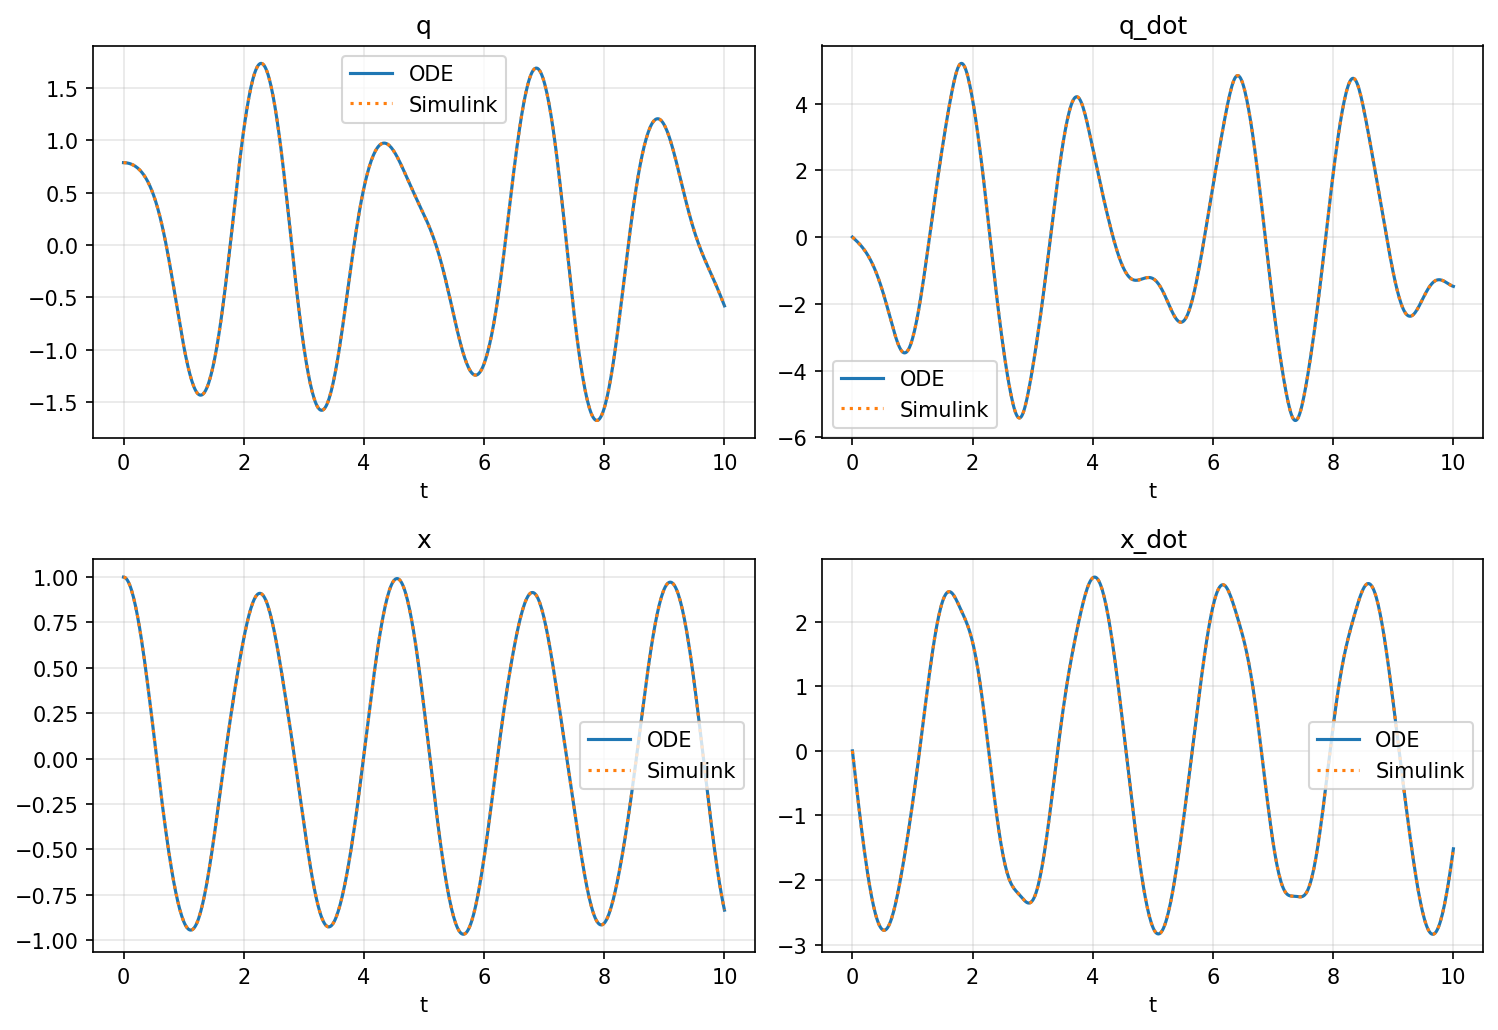
\includegraphics[width=\linewidth]{figures/cart_pendulum_simulation.png}
\end{minipage}
\caption{A nonlinear cart-pendulum-spring benchmark generated by \EqnToSim{}. Left: the readable v2 Simulink model, organized into per-state subsystems with explicit integrator-chain structure. Right: the corresponding Python ODE and Simulink trajectories for $(q, \dot{q}, x, \dot{x})$; the measured RMSE and maximum absolute error were $1.23\times10^{-9}$ and $2.12\times10^{-8}$, respectively.}
\label{fig:cartpendulum}
\end{figure*}

\section{Discussion}
The main engineering result is that determinism and usability did not need to be traded against one another. The narrow input language reduced ambiguity enough for every stage of the pipeline to be benchmarked precisely, while the readable backend made the final Simulink artifact inspectable by a human engineer. That combination is important in workflows where the diagram itself is part of the review, debugging, or handoff process.

The benchmark design also sharpened the capability boundary of the compiler. Rather than claiming support for arbitrary mathematical input, \EqnToSim{} makes the supported subset explicit and tests that subset aggressively. Adversarial cases are therefore useful outcomes, not embarrassments: they document where the compiler should stop, report a categorized error, and refuse to guess.

Finally, the readable backend suggests a practical bridge between symbolic compilation and model-based design. Equation-based languages and tools already demonstrate the power of declarative modeling \cite{fritzson1998modelica,fritzson2020openmodelica}. \EqnToSim{} shows that a narrower, deterministic equation frontend can still produce a block diagram that remains meaningful inside a Simulink-centered toolchain.

\section{Limitations}
\EqnToSim{} is intentionally not a general \LaTeX{} mathematics parser. It does not accept arbitrary environments, arbitrary macros, or general symbolic manipulation beyond the supported operator set. DAE-like systems, underdetermined formulations, overdetermined systems, and implicit nonlinear derivative couplings are rejected instead of being solved heuristically. Nonlinear systems bypass state-space realization, and hybrid or event-like logic is only accepted when it can be represented in the current deterministic operator boundary.

The backend currently assumes a local MATLAB and Simulink installation. That dependency is appropriate for the target workflow, but it limits portability compared with purely open-source simulation stacks. In addition, the synthetic benchmark generator samples from the supported operator families; it improves coverage, but it does not constitute an unbiased sample of all equations seen in industrial modeling practice.

\section{Conclusion}
This paper presented \EqnToSim{}, a deterministic compiler that turns restricted \LaTeX{} ODE systems into validated, readable Simulink models. The pipeline covers canonical symbolic compilation, graph lowering, direct ODE simulation, optional state-space conversion for linear systems, real Simulink model generation, signal extraction, and end-to-end numerical validation. The current benchmark suite demonstrates preserved correctness on the original 216-case synthetic benchmark, complete success on a 255-case full benchmark, and successful nonlinear Simulink generation on several harder coupled systems.

The results show that equation-to-Simulink compilation can be both trustworthy and inspectable when the language boundary is explicit and the backend is validated aggressively. Future work will extend the supported grammar, enrich runtime metadata, widen the hybrid-system boundary, and explore export paths to model-exchange standards such as FMI.

\bibliographystyle{asmeconf}
\bibliography{references}

\end{document}
